%%%%%%%%%%%%%%%%%%%%%%%%%%%%%%%%%%%%%%%%%%%%%%%%%%%%%%%%%%%%%%%%%%%
%%% Documento LaTeX 																						%%%
%%%%%%%%%%%%%%%%%%%%%%%%%%%%%%%%%%%%%%%%%%%%%%%%%%%%%%%%%%%%%%%%%%%
% Título:		Apéndice A
% Autor:  	Ignacio Moreno Doblas
% Fecha:  	2014-02-01, actualizado 2019-11-11
% Versión:	0.5.0
%%%%%%%%%%%%%%%%%%%%%%%%%%%%%%%%%%%%%%%%%%%%%%%%%%%%%%%%%%%%%%%%%%%%

\pagestyle{fancy}
\fancyhead[LE,RO]{\thepage}
\fancyhead[RE]{Apéndice} %
\fancyhead[LO]{\nouppercase{\rightmark}}

\chapter{Manual de uso de la aplicación funcional}

% \minitoc

% \section{Primera sección}

Esta aplicación funcional se inicia a través del terminal, por lo que la ejecución 
del programa en C será suficiente para la transmisión y recepción de los paquetes.

Primero se precompila el programa en C y la FPGA ejecutando el comando \textit{Make} tal 
y como se explicará más adelante. Luego en la línea de ejecución se elige la frecuencia
de muestreo, el esquema de señalización y el sistema de decisión para cargar el 
programa deseado en la FPGA.

En función de los parámetros que se elijan se cargaran diferentes programas, en concreto, 
\textit{bitstreams} que corresponden a cada codificación diferenciando entre los sistemas
de decisión. Los bitstreams disponibles son los siguientes siendo x el nombre del 
sistema de decisión deseado (hard, soft, viterbi).

\begin{itemize}
    \item bitstream\_pulsos\_alternos\_x.bit
    \item bitstream\_cancelacion\_pulsos\_x.bit
    \item bitstream\_4ppm\_x.bit
\end{itemize}

A continuación, se explica paso a paso como lanzar la aplicación suponiendo que los 
archivos mencionados previamente están copiados y en una carpeta accesible en el 
sistema de archivos de la Red Pitaya. 

Se abre un terminal en un PC conectado a la misma red local que la Red Pitaya, 
iniciamos una sesión SSH y navegamos hasta la ruta donde se encuentra el fichero
\textit{Makefile}. 

Una vez en la ruta ejecutamos el comando \textit{make}.

Posteriormente ejecutamos el programa introduciendo, a su vez, el modo de funcionamiento,
el bitstream que se va a cargar y el número de TAPs para definir la frecuencia de trabajo
mediante el siguiente comando:

\textit{./bin/test txrx soft\_4ppm 125}

Una vez hecho esto se verá en el terminal como se transmiten y reciben los paquetes.

Es importante destacar que el transceptor hardware está implementado para hacer uso del
puerto IN1 del ADC y el puerto OUT1 del DAC, por lo que para este prototipo la conexión
entre el transmisor y el receptor se deberá implementar tal y como se muestra en la
figura \ref{conex}.

\begin{figure}[ht]
    \centering
    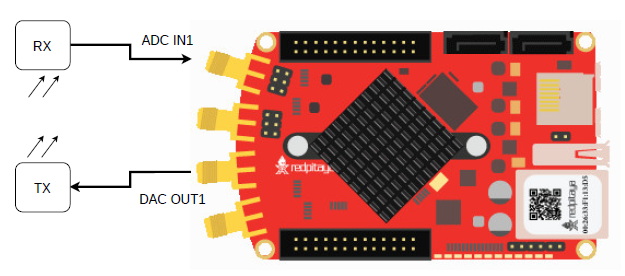
\includegraphics[scale=0.50]{./figuras/conexion_pitaya.png}
    \caption{\small{Conexión entre los conversores de la Red Pitaya para el prototipo 1.}}
    \label{conex}%
\end{figure}

\chapterend